\subsection{Children's polite speech understanding}
\label{sec:child}

Previously we have shown that adults in the US think about polite speech as reflecting a tradeoff between information transfer and face-saving. Would children reason likewise? Here we extend our tradeoff hypothesis to suggest that, starting at a young age, people distinguish between these goals and reason about the optimal degree of tradeoff (i.e. what is the nicest, most helpful thing to say) based on the speaker's intention, listener's need, and cultural expectations. Thus, adults and children should reason about polite language as broadly reflecting a tradeoff between information-saving and face-saving, although such understanding may mature over time. 

\subsubsection{Background}

There is not as much evidence collected for young children's understanding of polite speech (specifically white lies) as for children's production of polite speech. For example, children as young as 3 years start to tell white lies; they lie to the giver of an undesirable gift and say that the gift is nice \citep{talwar2007}. 

Interestingly, understanding of lies in general and motivations for white lies, is displayed in later years than production: 8- and 11-, but not 4-year-olds, demonstrate correct categorization of truths as truths and lies as lies \citep{bussey1999}; 7- to 11-year-olds rate lies as more positive in politeness than transgression contexts \citep{heyman2009}. However, no study has yet looked at how children spontaneously reason about motivations behind lies and truths, especially those related to the epistemic-social tradeoff that we are currently interested in. 

\subsubsection{Empirical test: Experiment 3}

To examine our hypotheses about children's polite language understanding, we would like to look at how children reason about speakers who speak truthfully but impolitely, or politely but untruthfully. To do this we propose a procedure that is based on the scenarios used with adults, but simplified: participants will be asked to read a story in which, for example, two speakers tasted yucky cookies and were asked how they liked it, either by the baker himself, or someone else. One speaker speaks truthfully (``the cookie was yucky'') and the other untruthfully (``the cookie was tasty''). Participants will then judge whether each speaker was telling the truth and whether she was nice or mean, and indicate whether they prefer to play with the truthful speaker or the untruthful speaker. This procedure has been piloted and has worked well in India, as well as other two sites of interest (Pilot findings are discussed in the next subsection).
 
{\bf Data collection procedure.} Participants will be recruited at children's museum and nursery/elementary schools in US. Across these three different sites, we will recruit three different age groups (3-4, 5-6, and 7-8-year-olds), with 24 participants per condition. Those who are not exposed to English at least 75\% daily will be excluded from data analysis. 

{\bf Design.} There are two independent variables: (1) listener type: whether or not the context was such that the `listeners' in our story asked about their own performance (e.g., cookie that they baked) or another, unknown person's performance (e.g., a cookie that was lying around for free); and (2) speaker type: whether the `speakers' in our story decide to tell a lie or truth about the performance. 

Each participant will be randomly assigned to one `listener' condition (i.e., whether the story is about listener's performance or someone else's) and will go through both `speaker' trials (i.e., speaker who tells a lie and speaker who tells the truth). Thus, the `listener' variable is a between-subjects, and the `speaker' variable is a within-subjects factor. There will be two sets of two speaker trials, and the order of the sets will be counterbalanced across subjects.

We will ask the following questions to participants: (1) In each trial, after telling the story of each speaker: ``Was [the speaker] in the story nice? Was she mean? Was she telling the truth?'' (the order of questions will be counterbalanced); (2) After one set of two trials, comparing two speakers, one who told a lie vs. one who told the truth: ``Who do you want to play with more, [polite speaker] or [honest speaker]?''

{\bf Analysis plan.} We will use a mixed-effects logistics regression model to analyze: (1) participants' rating for a given speaker's niceness/meanness/truth-telling; (2) comparisons of polite vs. honest speakers, as indicated by whom they ``want to play with.''

\subsubsection{Results from pilot work}

We have run pilot study of the proposed work, and Figure~\ref{fig:expt3} is an example analysis conducted on pilot data. We see an interesting developmental trend where 8-year-olds show similar patterns of niceness attribution to adults but it is not as much differentiated between honest and polite speaker, whereas 6-year-olds do not differentiate between the honest and polite speaker at all.

\begin{figure*}[t]
\begin{centering}
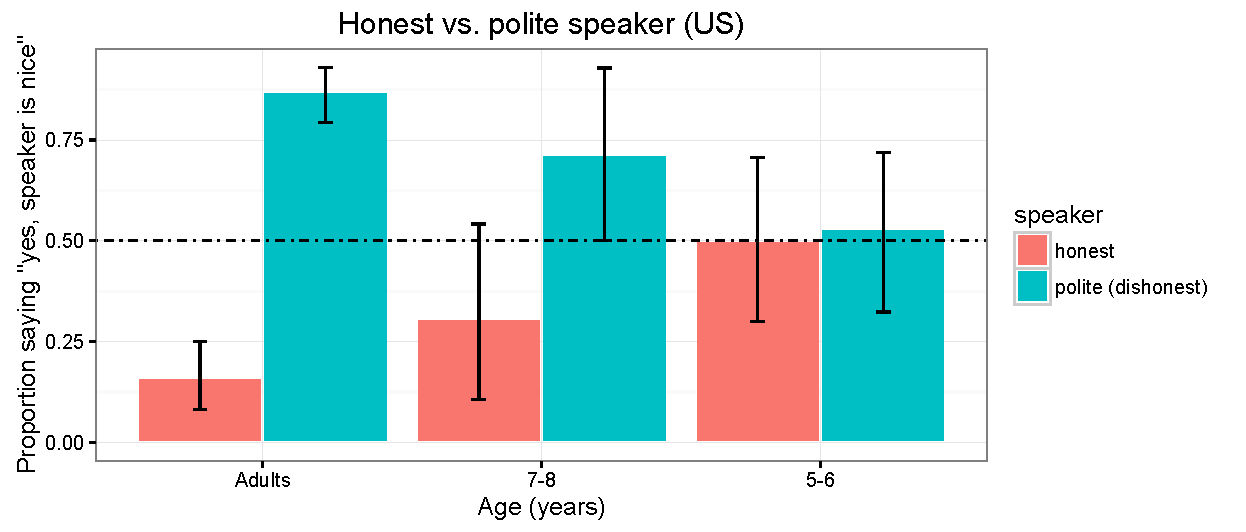
\includegraphics[width=\textwidth]{figures/exp3.pdf}
\caption{\label{fig:expt3} Results from Experiment 3 (pilot), for children's niceness judgment for honest versus polite (but dishonest) speaker. Error bars represent 95\% confidence intervals.}
\end{centering}
\end{figure*}


\subsubsection{Implications for the model}

Based on our pilot results, children seem to show similar patterns of inferences for honest versus polite speakers, in that they judge polite speaker as nice and honest speaker as not nice. However, this pattern is less clear in 6-year-olds, who do not differentiate between the two speakers. Interpreting these results, if this pattern holds, is possible in two ways: younger children have the same mechanistic process for evaluating the epistemic-social tradeoff to determine the speaker's social utility, but this is obscured due to some cause such as task demand, or younger children do not see the utterance as reflecting the epistemic-social utility at all. The former would be in favor of our model and its universal application, but further evidence (with greater statistical power) is needed to assess the model fit to the data.



%%% Local Variables: 
%%% mode: latex
%%% TeX-master: "desc"
%%% End

